\documentclass[10pt,conference,compsocconf]{IEEEtran}

\usepackage{hyperref}
\usepackage{graphicx}
\usepackage{xcolor}
\usepackage{blindtext, amsmath, comment, subfig, epsfig }
\usepackage{grffile}
\usepackage{caption}
%\usepackage{subcaption}
\usepackage{algorithmic}
\usepackage[utf8]{inputenc}


\title{CS-523 SecretStroll Report}
\author{Wicky Simon, Nunes Silva Daniel Filipe}
\date{April 2020}

\begin{document}

\maketitle

\begin{abstract}
  This project is split into three parts related to users privacy in the context of a location based service.
  In the first part we make use of attribute based credentials (hereafter ABC) and zero-knowledge proof to anonymously query a server for nearby points of interests (hereafter PoIs) and prove the ownership of a subscription. The second part is dedicated to the loss of privacy induced by IP-level metadata leak. The last part allows us to try to infer the location of users based on the eavedroppen metadata of their queries routed through Tor.
\end{abstract}

\section{Introduction}

The aim of the first part of this project is to build a privacy-friendly location based service called SecretStroll, which allows users to query a database about nearby PoIs while remaining anonymous. Since this service is not free, every query must provide the proof of an active subscription. Each PoI is part of a category such as \textit{Restaurant}, \textit{Office}, \textit{Dojo}, etc. Each of these categories is part of a subscription and users may have multiple of them, which leads to ABC. A user joining the service first registers himself with the categories he paid for and signs each of his queries anonymously, revealing only the categories he want to get PoIs from. In the following parts we assess remaining privacy issues and possible attacks as well as potential defences and their effectiveness.

\section{Attribute-based credential}
The base of the ABC scheme for this work is described in Section 6 of \cite{PS_Scheme}. This scheme has been used as follows : 
\begin{itemize}
    \item The messages mentionned in \cite{PS_Scheme} are attributes, representing categories of PoIs. The server creates a public key large enough to encode all of these attributes. 
    \item When a user wants to register, she commits to attributes she paid for, that will remain hidden. She uses a zero-knowledge proof (ZKP) to prove that she did so correctly. The server checks the proof, and sign this commitment that she will then use as credential.
    \item When a user makes a query, she choose the attributes (i.e the categories of PoIs) that she want. She then makes use of her credential to prove she has a subscription for the queried attributes, using a ZKP. She also uses this credential to sign a message representing her current location using the Fiat-Shamir heuristic described in \cite{FSheuristic} and detailed later.
\end{itemize}

In order to make the ZKP non-interactive, we use the Fiat-Shamir heuristic. The challenge that the prover would send is replaced by a cryptographic hash of all known values. During the registration, the challenge is composed of the committed attributes, the commitment used for the ZKP and the server's public. To sign the message for a query, it is simply added to the other values constituting the challenge. 

This overall approach leaks only the number of attributes chosen, but it is necessery for the server to correctly compute the ZKP. Otherwise, hidden attributes cannot be inferred and every credential is unique.

\subsection{Test}
The system is tested with six different tests : 
\begin{enumerate}
    \item \textit{test\_generate\_ca()} : The server's certificate generation is tested with a simple structure test, to see if all keys have the right lenghth.
    \item \textit{test\_credentials\_difference()} : Two requests are created with the same input parameters, a registration is perforemd with both of them and two credentials are created. To preserve anonymity, the requests and the built credential should be different. \\ Two credentials created from the same request should also be different.
    \item \textit{test\_tampered\_credential()} : A request with invalid credential should be rejected. In this test, a valid credential is tampered to be invalid.
    \item \textit{test\_correct\_credential()} : A request with a correct credential should be accepted.
    \item \textit{test\_correct\_credential\_no\_attributes()} : A request revealing no attributes should be valid.
    \item \textit{test\_wrong\_revealed\_attr()} : A request revealing unobtained attributes should be invalid.
\end{enumerate}
The effectiveness of these tests could be assessed using a standard metric such as branch coverage or coverage. However, these metrics are not complete and will not discover every bug present in the code.


\subsection{Evaluation}
The system is benchmarked in two parts, an offline part, which evaluate pure computationnal time and an online part which evaluate the communication time. The benchmark require the package \verb|pytest-benchmark| to be installed

\subsubsection{Offline benchmark}
The offline benchmark tests four features :
\begin{itemize}
    \item Key generation
    \item Credential issuance
    \item Message signing
    \item Signature verification
\end{itemize}
The result are shown in figure \ref{bench_fig}
and reported in table \ref{benchoffline}

\begin{table}[]
\centering
\begin{tabular}{|l|l|l|}
\hline
                                 & Median [ms] & Std Dev [ms] \\ \hline
test\_registration on i7         & 47.86  & 12.50   \\ \hline
test\_registration on i9         & 53.42  & 20.27   \\ \hline
test\_credential\_checking on i7 & 96.34  & 12.97   \\ \hline
test\_credential\_checking on i9 & 96.01  & 2.63    \\ \hline
\end{tabular}
\caption{ABC system online benchmark on 500 rounds}
\label{benchonline}
\end{table}

\begin{table}[]
\centering
\begin{tabular}{|l|l|l|}
\hline
                                 & Median [ms] & Std Dev [ms] \\ \hline
test\_key\_generation on i7      & 26.73  & 1.63    \\ \hline
test\_key\_generation on i9      & 25.45  & 1.25    \\ \hline
test\_credential\_checking on i7 & 45.32  & 3.84    \\ \hline
test\_credential\_checking on i9 & 38.86  & 2.04    \\ \hline
test\_credential\_showing on i7  & 46.92  & 5.23    \\ \hline
test\_credential\_showing on i9  & 39.56  & 2.18    \\ \hline
test\_credential\_issuance on i7 & 44.37  & 4.26    \\ \hline
test\_credential\_issuance on i9 & 39.87  & 1.90    \\ \hline
\end{tabular}
\caption{ABC system offline benchmark on 500 rounds}
\label{benchoffline}
\end{table}

\subsubsection{Online benchmark}
The online benchmark tests two features :
\begin{itemize}
    \item Registration
    \item PoIs request
\end{itemize}
Note : This benchmark has requirements. Follow the instructions at the beginning of \textit{benchmark\_net.py}.

The result are shown in figure \ref{bench_fig}
and reported in table \ref{benchonline}
\begin{figure}
    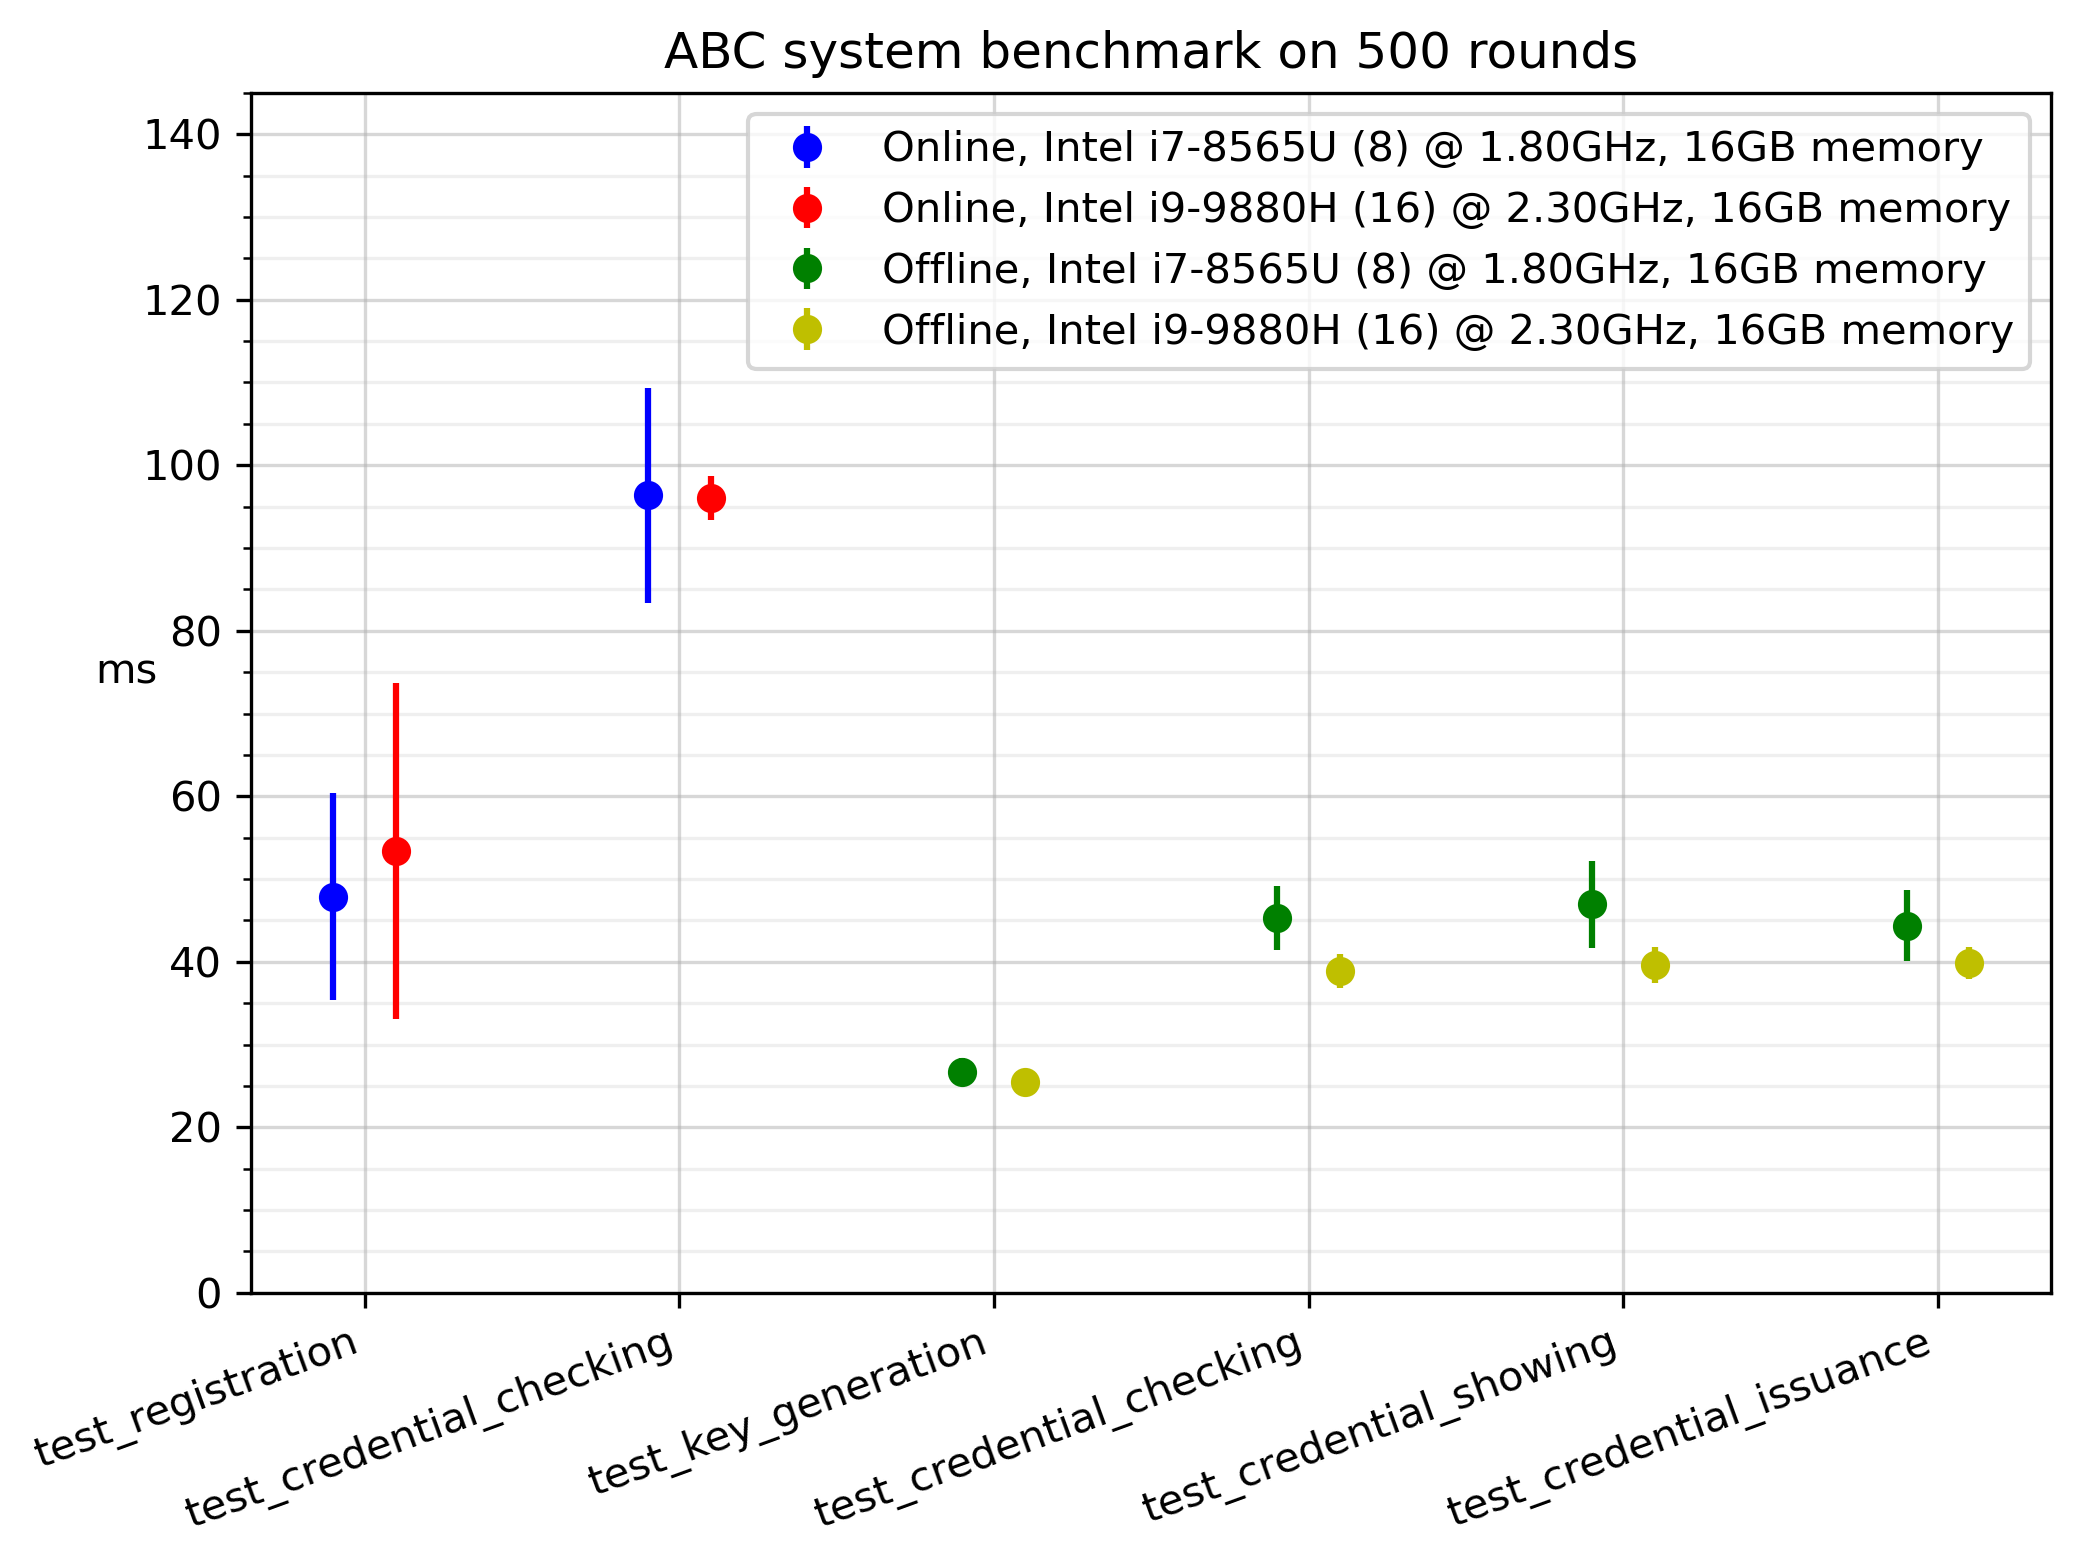
\includegraphics[width=\columnwidth]{ABC_system_benchmark_on_500_rounds.png}
    \caption{ABC system benchmark on 500 rounds}
    \label{bench_fig}
\end{figure}


\section{(De)Anonymization of User Trajectories}

\subsection{Privacy Evaluation}
We evaluate the privacy risks using simulated data of two hundred users who made use of the application hundred times each in average over twenty days. We assume that no mechanism to hide any kind of data is used, i.e. data is sent in cleartext inside standard IP packets. Any malicious adversary could hack the application servers or sniff the network between a user and the server in order to retrieve similar datasets which include IP addresses, locations, query types, timestamps and responses. According to \cite{dont}, the IP address or a set or IP addresses are relevant attributes because they can be linked to a given user since they are persistent for a certain duration. Moreover, combining IP addresses with location and time data makes sense since users often keep their habits that they may share with very few people \cite{on}, i.e. they may work during the day at their office, be back home in the evening and do an activity at some specific location. Therefore, we expect this implementation to leak senstive informations about the users. As a proof of concept for breaching users privacy, we try to infer work and home locations of users as well as habits in their activities.

We build our attacks in a constructive way, starting by learning general tendencies about the users, then, we focus on one specific user in order to learn how far we can go with breaching breach its privacy.

As stated before, home and work are sensitive locations because they allow to identify users. In order to learn about them, we go through all users queries and check if users queries locations correspond to home types locations such as \textit{appartment blocks} or \textit{villas} as well as work types locations such as \textit{offices}, \textit{laboratories} or \textit{companies}. It turns out that each user has one location of each from where it does the majority of its queries which allows us to draw a map linking IP addresses to their corresponding home and work locations. Moreover, \ref{share_fig} confirms our concern about users anonymity once their home and work locations would leak in the given setup. The logarithmic scale clearifies the orders of magnitude between people who share or not these POIs showing that the majority of the users have a tuple home and work location that they share with very few people as presented in \cite{on}.

\begin{figure}
  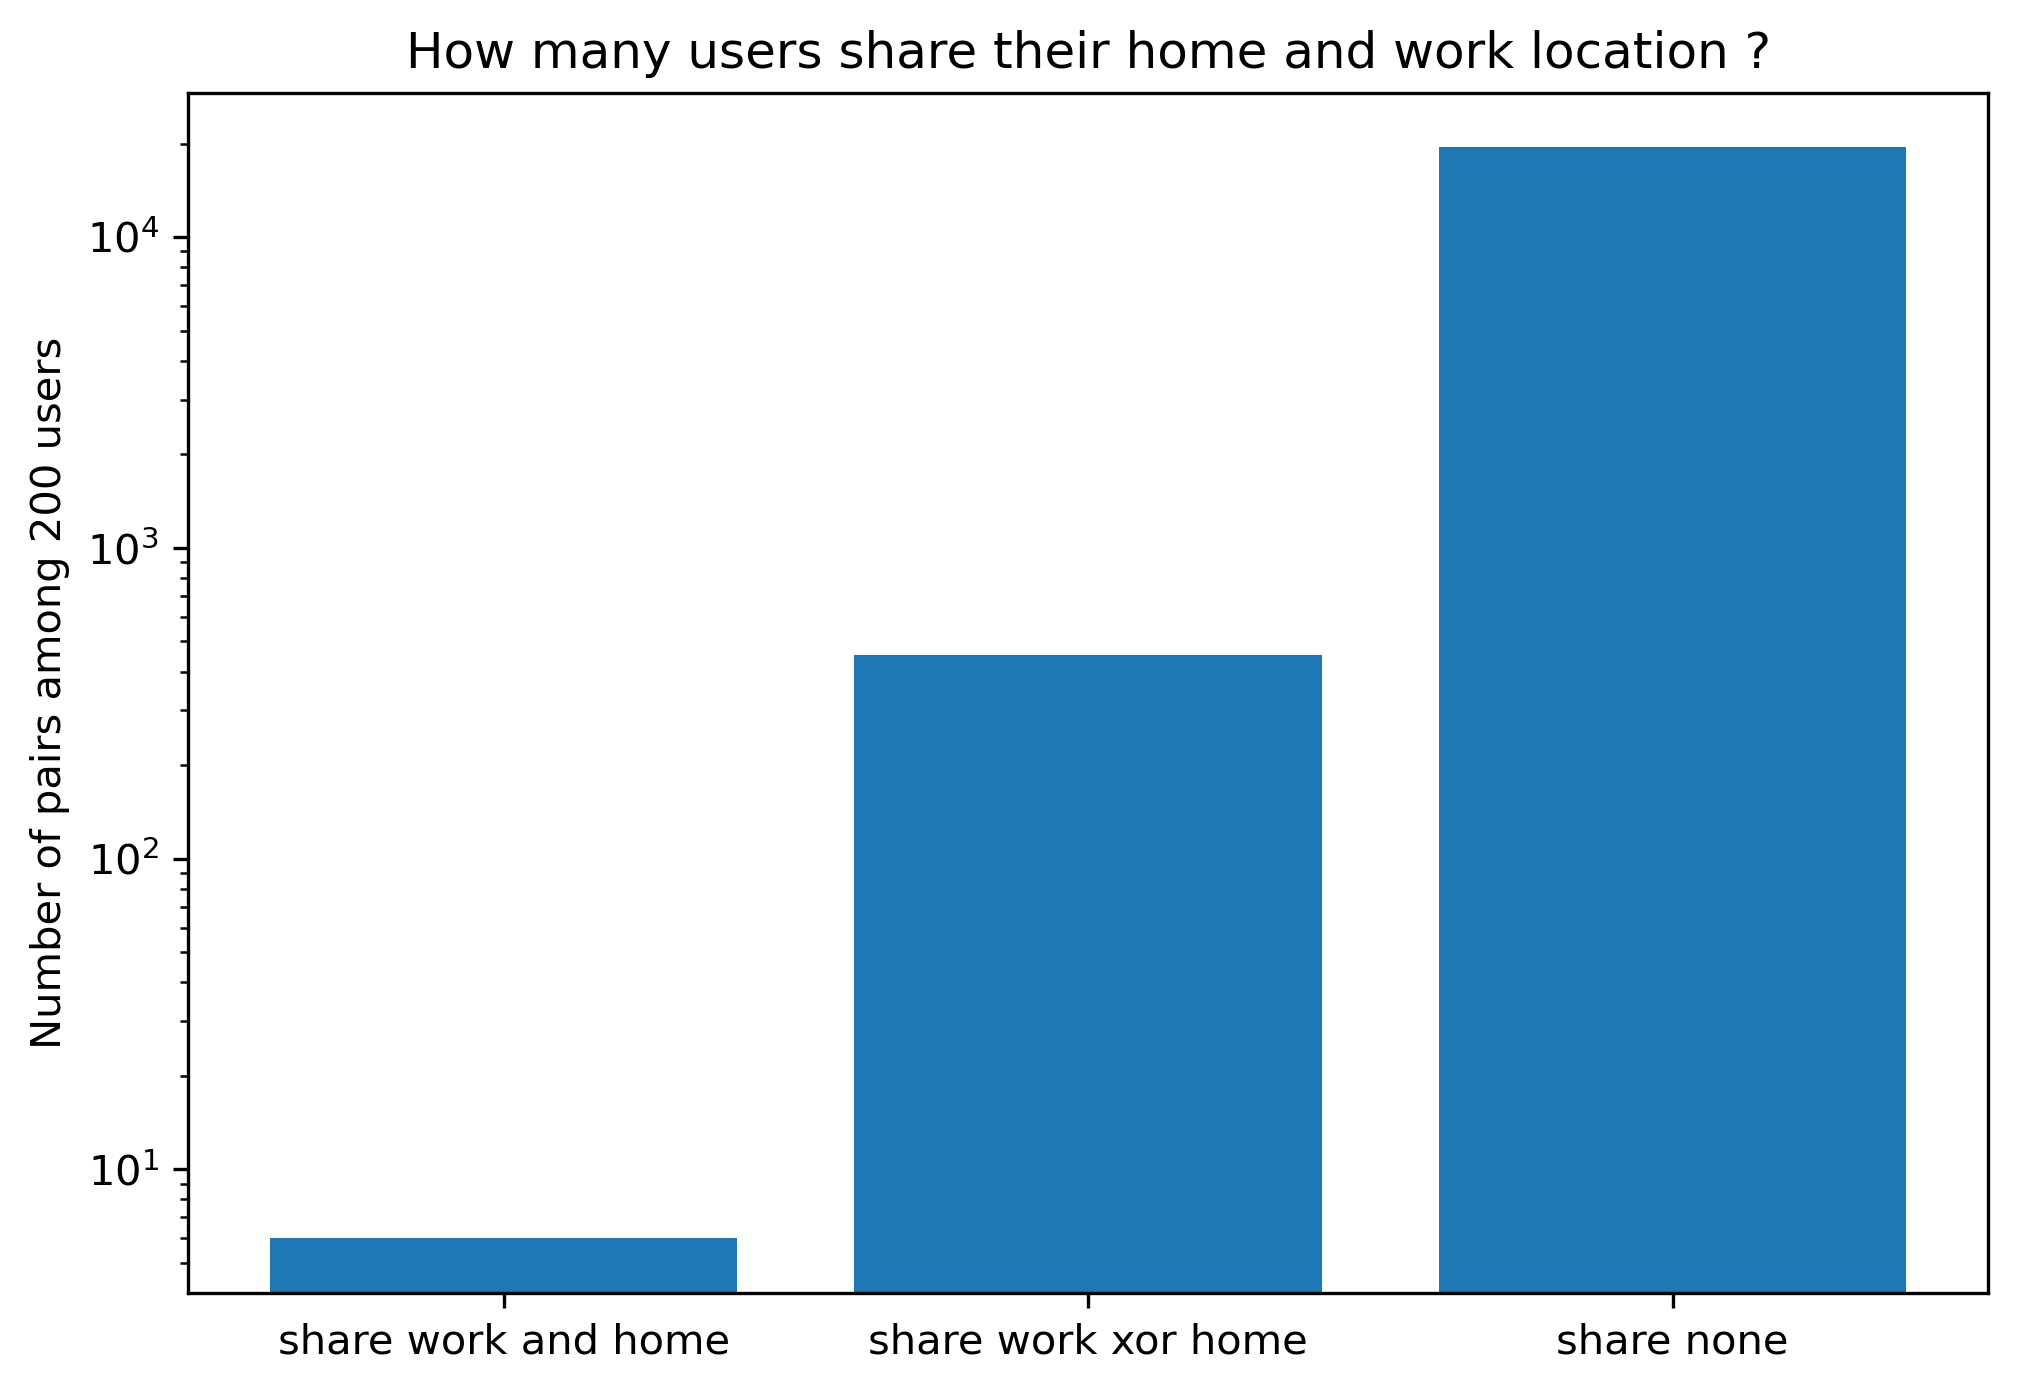
\includegraphics[width=\columnwidth]{share.png}
  \caption{Comparison of how people share their main POIs}
  \label{share_fig}
\end{figure}

Then, we analyze when users make use of the app from their home and work locations. On the one hand, we observe that they use it regularly on a daily basis from home. On the other hand, we can see that they query the service from their work location only during weekdays, which is compatible with not being on their work location on the weekend. Moreover, we consider when the app is used during the day on weekdays in \ref{when_fig}. This shows that users likely spend their day at work while being at home at the end of the day. This short analysis gives a great understanding of users habits even though the presented results seem trivial.

\begin{figure}
  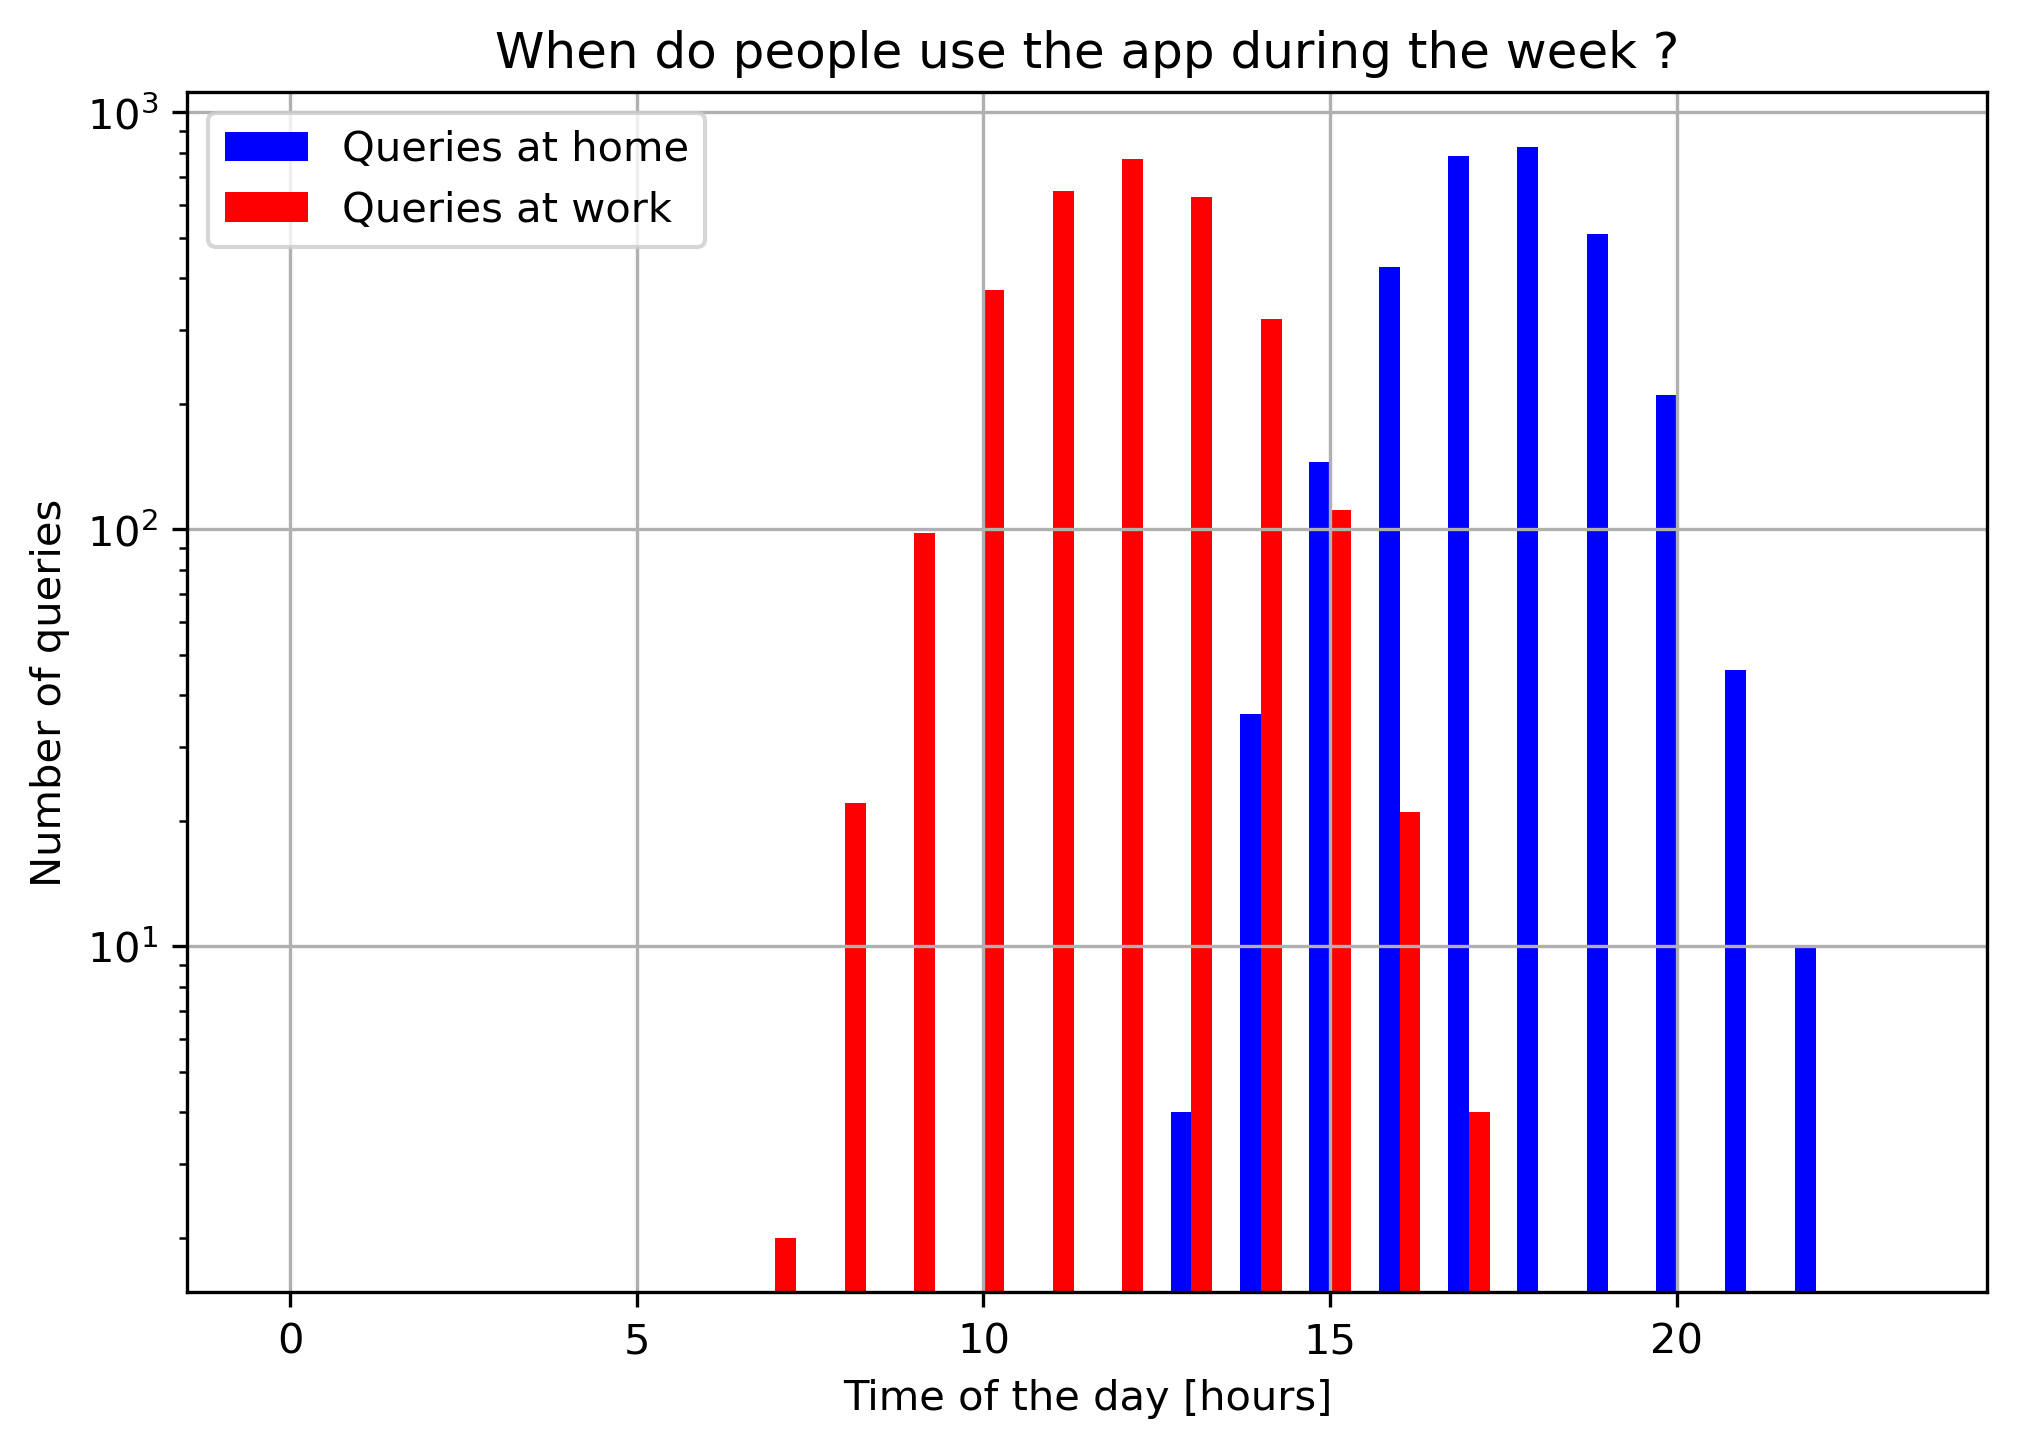
\includegraphics[width=\columnwidth]{when.png}
  \caption{User habits}
  \label{when_fig}
\end{figure}

Finally, we focus on breaching privacy of a chosen user to assess if we can learn more about a given user than general tendencies. Our results are condensed in the graph presented in \ref{random_fig} that shows how user moves as a function of time. We are able to determine where the user lives and works making use of our previous findings. From that, we can see how this user's life is centered around its home and work locations. In fact, it goes back and forth its home and work during the week while its trajectory take completely different paths on the weekends. Applying similar techniques for other POIs types allows us to learn about this user's favorite restaurant and when it used to eat there. Then, grouping \textit{bars} and \textit{clubs} as entertaining activities opposed to \textit{gym} and \textit{dojo} which can be considered quiet ones, we deduce that this particular user is more into the former ones which are located close to its home. He basically goes to the gym on the weekends as we can see these spiky outliers in \ref{random_fig}.

To sum up, we assessed how we could breach users privacy by analyzing either general habits about the users or more personal ones by focusing on specific users. This leads us to conclusive results regarding our initial references and expectations leveraging simple algorithms such as matching users queries locations with meaningful POIs. The cost would depend on how close and severely someone wants to attack a specific user. As shown earlier, we can either keep it very general and learn about tendencies or focus on a given user. For future attack, we may be interested to evaluate how the current POIs locations may be related to the next queries in order to understand better users behaviour. For example, how likely is it that a user wants to go for a beer after work compared to after gym ?

\begin{figure}
  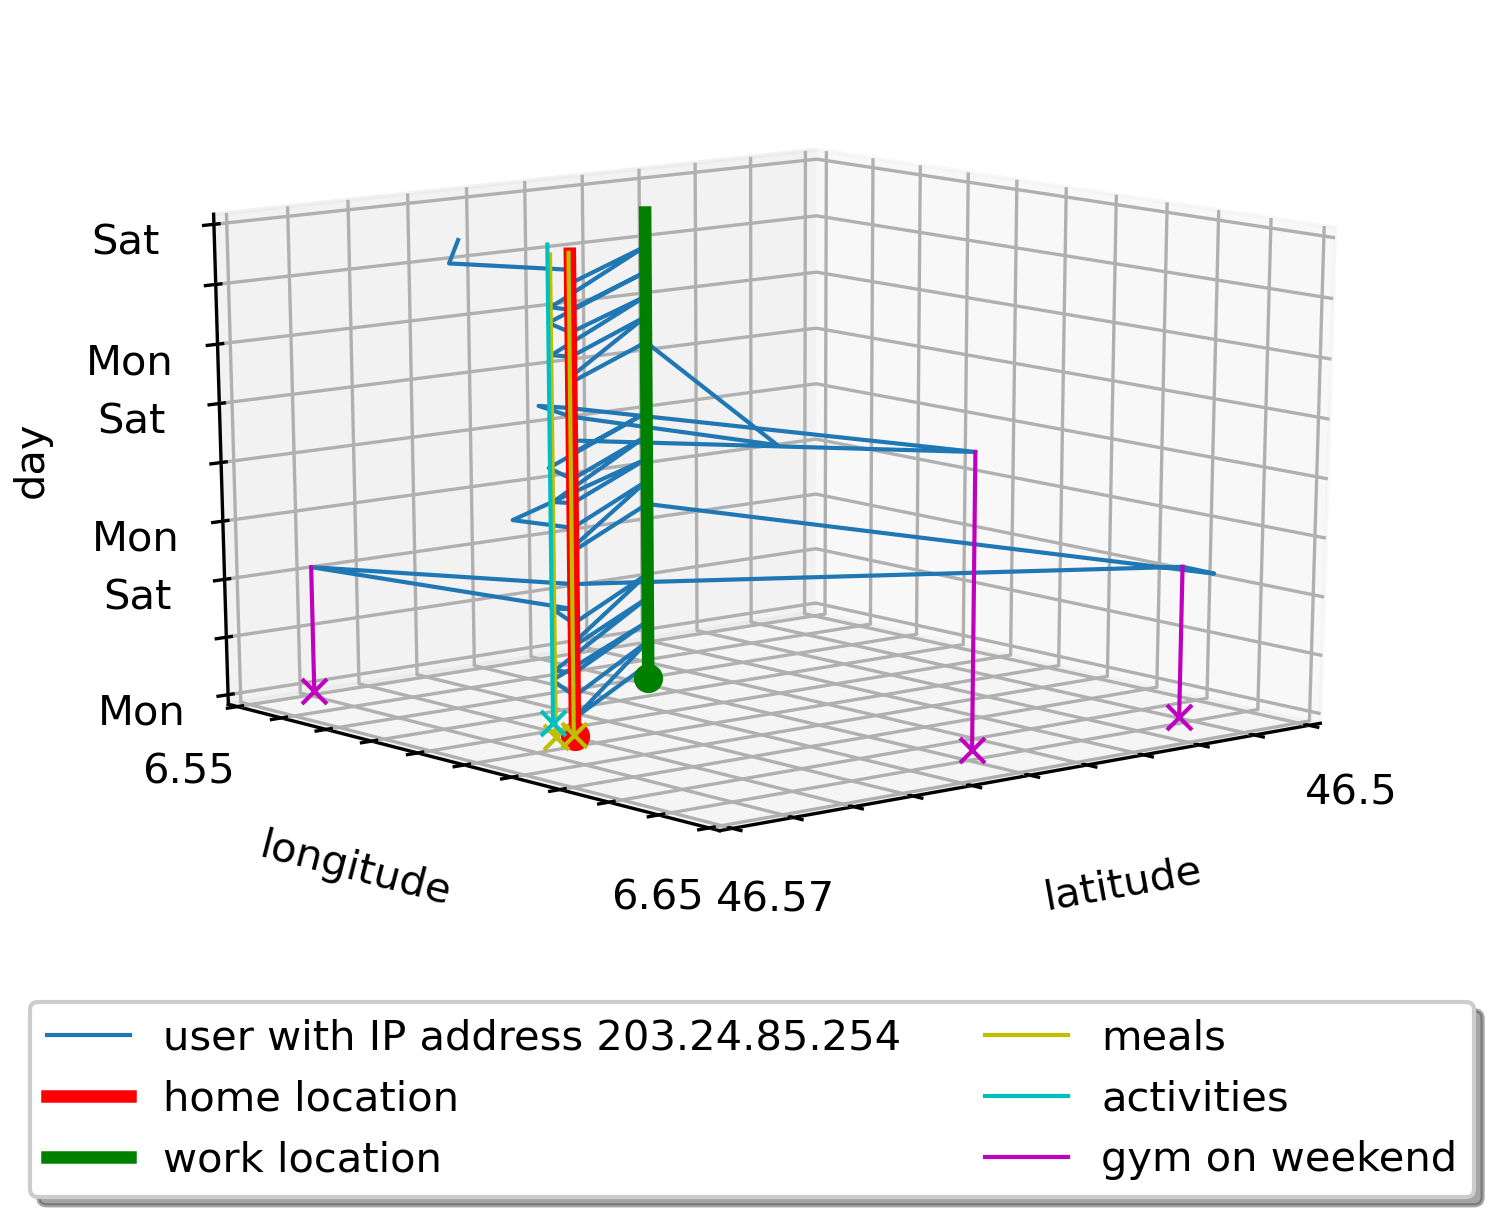
\includegraphics[width=\columnwidth]{random.png}
  \caption{Monitoring of a randomly chosen user using collecting data}
  \label{random_fig}
\end{figure}

\subsection{Defences}
Now that assessed that we assessed the privacy issues of this app, we suggest one simple and lightweight client-side defence that would help improving it.

We remember that the purpose of this app is to suggest POIs of a given type in the grid-based vicinity of the user. According to the specifications and \cite{deg}, an actual grid cell is of a similar scale of a city whose side measures a few kilometers. However, the collected location infomartions has artificially ridiculous precision considering that eight decimal places is precise up to a millimeter\cite{relevant_xkcd}. For this, we can suggest generalization by reducing the precision of the queries locations to two decimal degrees. In fact, it is still sufficiently precise to determine in which grid cell the service should do its recommendation in this setup. A cleaner way of implementing this would be by allowing users to download the grid cells locations and dimensions so that when querying the server they would transmit the minimum of information required to keep its utility, i.e. a cell ID.

This defense aims to protect the privacy related to the exact location of each query. In our previous attack, we take advantage of being able to map queries locations to the exact corresponding POIs. In this case, we are restricted to the POIs in the actual grid cell whose sizes are crucial and difficult to optimize. For example, if there are only bars in a given grid cell then if a user who would query the service from there would be likely doing it from a bar. Cells should then have k-anonymity, l-diversity and t-closeness to optimize this aspect so that if a user is querying the service from a grid cell, we should not be able to say from which POI nor which kind of POI the user is doing it from. However, this only provides only a probabilistic fine-grained location protection, assuming grid cells have the correct properties, that still may be defeated. A strategic adversary could learn about general habits of users but it would be harder to infer as much detail as we did in our attack, i.e. exact home and work locations as well as wenkend activities or favorite restaurant. For example, it could still observe home and work rides based on grids cells and timestamp but should not be able to say which exact POI inside the given cell it is own.

Our defence machnism does not affect utility from the results perspective. User will be able to receive the same suggestions as without this mechanism. In fact, we limit the user's outgoing information to what is strictly necessary to achieve the same utility in this setup. However, having to process this information locally to deduce the cell ID would require the user to have these grid properties stored on its phone. When travelling to a new region, the user may not have the coordinates available to derive the right cell ID which could limit the utility by requiring additional bandwith.

Making use of this mechanism allowed us to turn the previous anonymity set of peole sharing at least of home or work location from 457 pairs of users to 1186 pairs of user. This poor improvement can be justified mostly by the simplicity of the mechanism as well as by the non uniform distribution of POIs in the specified grids. The used mechanism of strongly utility oriented since it does not improve the privacy reasonably but preserves a similar utility with negligeable overhead. For this mechanism to be more efficient, strong assumptions about how grid are drawn, i.e. increase grid cells in order to include more POIs in each and provide better anonymity. This would also imply a utility decrease as the notion of vicinity my become too broad for the user to find POIs nearby. An alternative that would be interesting to assess in a future work would be replacing actual location informations by dummy ones. POIs are already established, we can make use of their semantic to compensate the usual lack of plausibility often experienced by this mechanism, i.e. a user could replace its home location by an other one located nearby in order to prevent the leak of it.

\section{Cell Fingerprinting via Network Traffic Analysis}

\subsection{Implementation details}
\subsubsection{Data collection}
The data was collected using the \verb|capture.sh| script. It loops through all the cells, queries the server for it, and dump the traffic between the client and the proxy. The traffic is captured there to avoid parasitic traffic. Each cell was queried 10 times, for a total of 1000 queries.

The file \verb|pcap.py| contains various function, to check the correctness of the capture file, aggregate features and save them in a csv to store them and prepare the data for our classifier. Note that since we used these functions for data collections only, they are not designed to be robust and might crash if the format requirements are not met. 

The data fed to the classifier consists of the bytes of the packets header converted to an integer between 0 and 255. Each of these values is normalized to be in the $[0,1]$ range. To allows the classifier to extract some structure, we kept only the headers who were 66 bytes long, which was the most frequent. We also kept only the first 400 packets, to have a reasonable training time. All capture smaller than 400 packets are simply padded with 0 bytes. These numbers are totally arbitrary and could be tuned if the available hardware was more powerful.

\subsubsection{Classification}
Inspired by \cite{tor_classification} and \cite{dl_encrypted}, we implemented our classifier as a standard convolutionnal neural network. Its architecture is shown in figure \ref{model_arch} and is constituted of the following layers:

\begin{enumerate}
    \item Convolution
        \begin{itemize}
            \item Input channels: 1
            \item Output channels: 32
            \item Kernel size: 66
            \item Stride: 66
        \end{itemize}
        The parameters of this layer allows the classifier to extract per packet features.
    \item Max-Pool: 
        \begin{itemize}
         \item Kernel size: 2
        \end{itemize}
    \item ReLu
    \item Convolution
        \begin{itemize}
            \item Input channels: 32
            \item Output channels: 64
            \item Kernel size: 3
        \end{itemize}
    \item ReLu
    \item Fully connected
        \begin{itemize}
            \item Input size: 12672
            \item Output size: 500
        \end{itemize}
    \item ReLu
    \item Fully connected
        \begin{itemize}
            \item Input size: 200
            \item Output size: 500
        \end{itemize}
\end{enumerate}

\begin{figure}
    \centering
    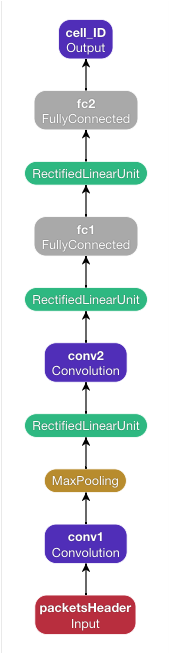
\includegraphics[scale=0.5]{model.png}
    \caption{Architecture of the CNN classifier \textsuperscript{1}}
    \small\textsuperscript{1} The software is available on Github under a MIT license (\url{https://github.com/mlajtos/moniel}).
    \label{model_arch}
\end{figure}
The training is done with 50 epochs, the cross-entropy is used as loss function and the \textit{Adam optimizer} as optimizer. As we used 10-fold cross-validation, the training dataset is constituted of 900 samples, the test dataset contains 100 samples.



\subsection{Evaluation}
After a 10 fold cross validation, the results are represented in table \ref{test_error}.

\begin{table}
    \centering
    \begin{tabular}{|c|c|}
        \hline
        Iteration & Error rate      \\
        \hline
        1      & $66\%$  \\
        \hline
        2      & $81\%$  \\
        \hline
        3      & $68\%$  \\
        \hline
        4      & $54\%$  \\
        \hline 
        5      & $74\%$  \\
        \hline
        6      & $68\%$  \\
        \hline 
        7      & $86\%$  \\
        \hline
        8      & $73\%$  \\
        \hline 
        9      & $83\%$  \\
        \hline
        10      & $80\%$  \\
        \hline      
    \end{tabular}
    \caption{Test error rate for each iteration}
    \label{test_error}
\end{table}

The final average is $73.3\%$ error rate, with a standard deviation of $9.18\%$.

\subsection{Discussion and Countermeasures}
At first sight, it seems that our classifier is quite bad. However, considering the number of possible classes, if we were guessing at random, we would have an error rate of $99\%$. This classifier allows us to improve our confidence approximately 26 times! Even by using Tor, our anonymity is not that protected. It is also important to note that this classifier was trained using a relatively small dataset, and low computationnal power. With more time and more powerful processing power, this result can surely be improved a lot.

Finding countermeasures to such a tool is extremely difficult. Machine Learning tries to extract structure in the data, and even when there is no structure at all, as seen in class, we can train an algorithm to detect this lack of structure. 

\bibliographystyle{IEEEtran}
\bibliography{bib}

\clearpage
We also enjoyed to make memes about this crazy project.
\begin{figure}[h]
  %\caption{Meme 1}
  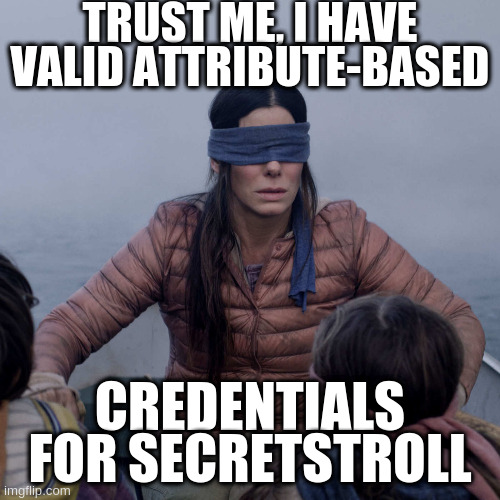
\includegraphics[width=0.3\textwidth]{meme/pets_meme_1.jpg}
\end{figure}
\begin{figure}[h]
  %\caption{Meme 2}
  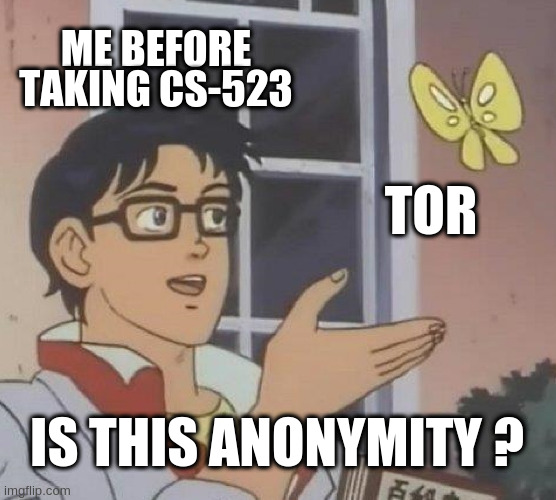
\includegraphics[width=0.3\textwidth]{meme/pets_meme_2.jpg}
\end{figure}
\begin{figure}[h]
  %\caption{Meme 3}
  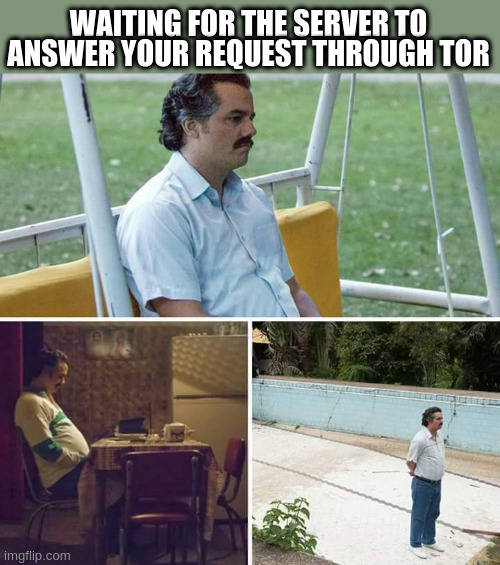
\includegraphics[width=0.3\textwidth]{meme/pets_meme_3.jpg}
\end{figure}
\begin{figure}[h]
  %\caption{Meme 4}
  
\includegraphics[width=0.3\textwidth]{meme/pets_meme_4.jpg}
\end{figure}
\begin{figure}[h]
  %\caption{Meme 5}
  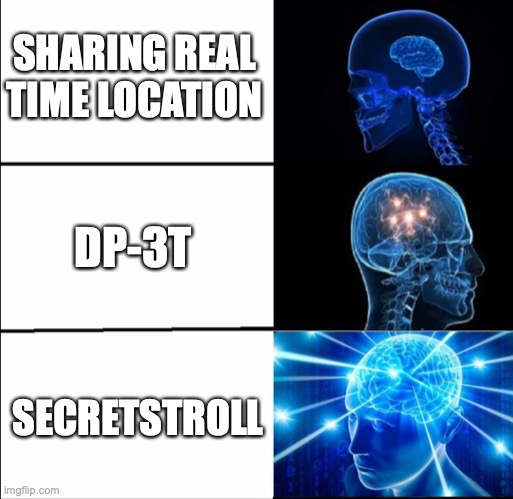
\includegraphics[width=0.3\textwidth]{meme/pets_meme_5.jpg}
\end{figure}
\begin{figure}[h]
  %\caption{Meme 6}
  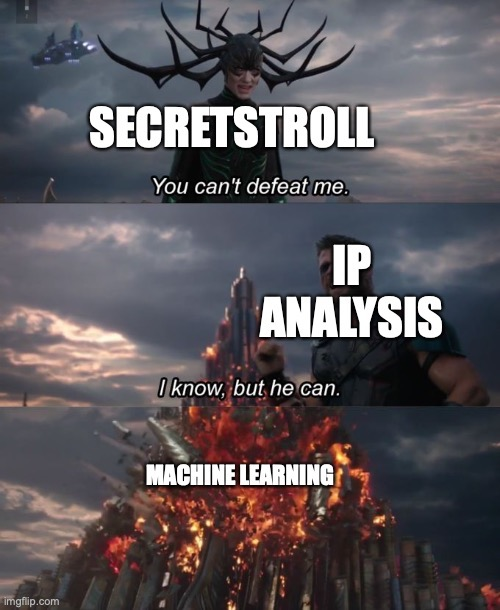
\includegraphics[width=0.3\textwidth]{meme/pets_meme_6.jpg}
\end{figure}

\end{document}
